\documentclass[a4paper,10pt]{article}
\usepackage[utf8]{inputenc}

\usepackage[english]{babel}
\usepackage[utf8]{inputenc}
\usepackage[top=7em, bottom=4em, left=5em, right=5em]{geometry}
\usepackage{mathptmx}
\usepackage{blindtext}
\usepackage{enumitem}
\usepackage{amsmath}
\usepackage{indentfirst}
\usepackage{graphicx}
\graphicspath{{figures/}}

\title{Relatório Final \\ Machine Learning}
\date{September 17,2018}
\author{Susana Bouchardet e Rebeca Bordini}

\linespread{1.5}
\begin{document}
\maketitle

\section{Introdução}

O problema de reconhecimento de dígitos é uma problema tradicional para validação de algoritmos de machine learning. O dataset mais tradicional para esse problema é o MNIST \cite{lecun-mnisthandwrittendigit-2010}, um dataset de digitos escritos a mão.

Originalmente esse dataset foi criado com o objetivo de criar um sistema de reconhecimento de digitos para reconhecer os números do \textit{zip-code} em cartas. Mas ele se tornou popular para validar modelos e algoritmos de reconhecimento de imagem. 

Nesse trabalho o objetivo é, utilizando esse dataset, experimentar diferentes algoritmos e técnicas para solucionar o problema. Para esse curso queremos encontrar uma solução com maior acurácia possiível. 

\section{Descrição do problema}

Para compreender melhor, vamos entender a descrição formal do problema. O problema proposto é um problema de aprendizado supervisionado, ou seja, temos dados já classificados e desejamos aprender uma maneira de classificar novos dados de maneira automática.

Para compreender melhor, vamos entender qual o \textit{Input} do modelo ($x$) e o \textit{Output} ($y$).

\begin{enumerate}
 \item [\textit{Input}:] 
 
 No caso desse problema, os \textit{inputs} são imagens  de $28\times 28$ pixels, com um canal. 
 
 Quando falamos de imagem, canal são as cores usadas para formar a imagem. Imagens coloridas tem normalmente 3 canais: Vermelho, Verde e Azul. No caso dos dados de \textit{input}, temos apenas um canal por se tratar de uma imagem em preto e branco. 
 
 Cada imagem pode ser descrita como uma matriz de $28$ linhas e $28$ colunas, onde o valor em cada célula representa a intensidade do pixel. A intensidade de cada pixel é um valor inteiro de $0$ a $255$, onde $0$ representa a cor preta e $255$ a cor branca.
 
  \item [\textit{Output}:] Dado o \textit{input} descrito acima, o modelo deve retornar qual número esta desenhado na imagem. Como cada imagem contém apenas um dígito, o problema é um problema de classificação com 10 classes: $0$, $1$, $2$, $3$, $4$, $5$, $6$, $7$, $8$ e $9$.
\end{enumerate}

\newpage

\begin{figure}[h]
        \centering
        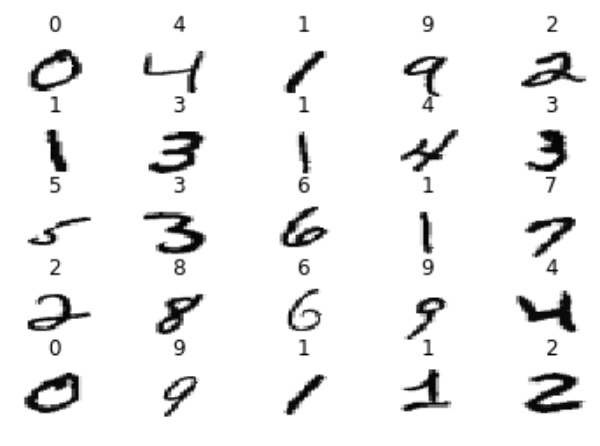
\includegraphics[width=10cm]{dataset_example.png}
        \caption{Exemplos dos dados disponíveis no dataset}
        \label{fig:exemploDataset}
\end{figure}

A figura \ref{fig:exemploDataset} mostra os dados disponíveis no dataset. Cada imagem é uma represnetação grafica dos \textit{inputs}. Sobre cada imagem existe o número que representa a classe associada a imagem, e que também é o \textit{output} esperado do modelo.

\section{Métrica de avaliação}

Varios artigos \cite{FredAgarap2017, Mahmoud2014, Sharma2015, Saavedra2014} utilizam a acurácia como métrica para avaliar o resultado de um modelo para solucionar esse problema. Por esse motivo decidimos então utilizar a acurácia como métrica.

A acurácia é uma métrica para classificadores que mede a taxa de acerto de um classificador. Seja $\hat{y_i}$ o valor predito pelo classificador e $y_i$ o valor real do i-ésimo exemplo, podemos descrever o calculo da acurácia como 

\begin{equation} \label{eq:acc}
 acc(y,\hat{y}) = \frac{\#\{\hat{y}_i | \hat{y}_i = y_i\}}{\#\{y_i\}}.
 \end{equation}

Pela equação \ref{eq:acc} é possível notar que o valor de $acc$ varia entre $0$ e $1$, de maneira que é $0$ se errar todas as classificações e $1$ se acertar todas as classificações. 

\section{\textit{Baseline} e \textit{state-of-the-art}}

A métrica para medir a performance do modelo, nesse caso, é a acuracia. Vamos usar dois valores como referência para julgar os modelos desenvolvidos nesse trabalho: um \textit{baseline} e a acurácia do \textit{state-of-the-art}.

\subsection{\textit{Baseline}}

O \textit{baseline} é a acurácia do classificador mais simples para resolver esse problema. Nesse caso, foi desenvolvido um classifidor randomico que classifica as entradas aleatóriamente de acordo com a distribuição das classes no dataset de treinamento. 

\begin{figure}[h]
        \centering
        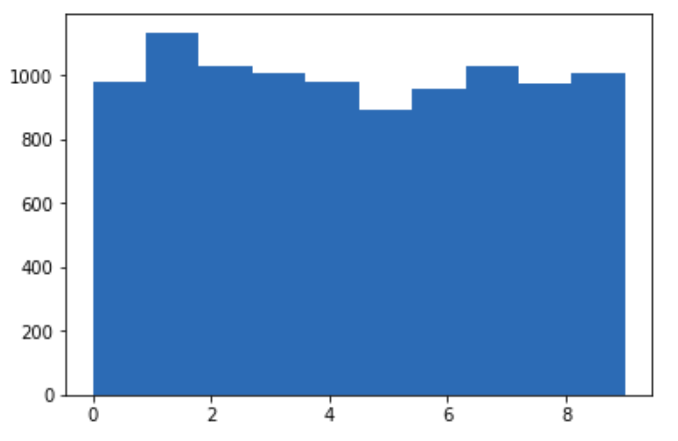
\includegraphics[width=10cm]{distribuicao.png}
        \caption{Distribuição dos dados de treinamento por classe}
        \label{fig:distribuicao}
\end{figure}

De acordo com a figura \ref{fig:distribuicao}, a quantidade de exemplos por classe é bem proxima. Baseado nisso, o classificador aleatório tem a mesma probabilida de sortear qualquer classe. Como o problema envolve $10$ classes, então cada classe tem a probabilidade $\frac{1}{10}$ de ser sorteada pelo classificador aleatório.

Para esse classificador obtemos um valor de acurácia de 0.1009

\subsection{\textit{State-of-the-art (SOTA)}}

O \textit{SOTA} atual é um comitê de modelos com 35 modelos \cite{DBLP}. Esses modelos são Redes Neurais Convolucionais (CNN). 

\begin{figure}[h]
        \centering
        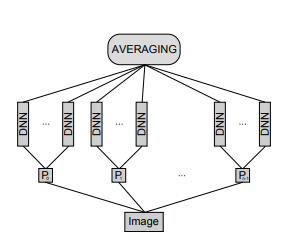
\includegraphics[width=10cm]{sota.png}
        \caption{Imagem retirada de \cite{DBLP} que mostra a arquitetura da solução proposta}
        \label{fig:sota}
\end{figure}

Na figura \ref{fig:sota}, o \textit{input} é o nó inferior. Esse nó é distribuido para $P_0, P_1, \dots e P_{n+1}$, que representam a etapa de pré-processamento. Cada etapa de pré-processamento alimenta uma ou mais redes neurais (DNN). Por fim, cada rede neural gera sua classificação, mas a classificação final é resultado da média dos resultados das redes neurais.

Com essa técnica, foram criadas 35 redes neurais convolucionais, e esse comitê de modelos obteve $0.9977$ de a acurácia.

\section{Modelos}

Nessa secção iremos descrever os modelos tentados, como os algoritmos funcionam e seus respectivos resultados. 

\subsection{Árvore de decisão}

O primeiro modelo testado foi uma árvore de decisão. Como o projeto foi desenvolvido ao longo da disciplina de machine learning, aplicamos parte do que aprendemos em seu desenvolvimento. O primeiro contúdo dado foi árvore de decisção. 

A árvore de decisção é um argoritmo de machine learning que tem como objetivo encontrar as regras que podem dividir melhor os dados de treino de acordo com suas classes. 

O dataset é disponibilisado em duas partes: treino e validação. Do dataset de treino, nós separamos 80\% do dado para de fato ser usado no treino e 20\% para ser usado como teste.

\begin{table}[h!]
\centering
\begin{tabular}{l||l}

            &   Acurácia    \\ \hline
Treino      &   1           \\ \hline
Teste       &   0.8705      
\\ \hline
Validação   &   0.874
\end{tabular}
\caption{Métricas obtidas no modelo gerado pela Árvore de decisão}
  \label{tab:metrica_dt}
\end{table}

O modelo gerado por esse algoritmo obteve a acurácia mostrada na tabela \ref{tab:metrica_dt}. É possível notar pela acurrácia obtida pelo daod de treino que o modelo aprendeu exatamente a classificação do treino. Isso demonstra que o algoritmo aprendeu o dataset, não a tarefe.

\subsection{DNN}

Outro algoritmo testado foi uma rede neural profunda (DNN). Nesse caso a arquitetura testada foi com apenas duas camadas ocultas, a primeira com 50 neurônios e a segunda com 25 neurônios. Todas as camadas eram totalmente conectadas.

Assim como nos modelos anteriores, temos os dataset separado em treino, teste e validação. A cada época de treinamento avaliamos a acurácia no dataset de test. 

\begin{table}[h!]
\centering
\begin{tabular}{l||l}

            &   Acurácia    \\ \hline
Treino      &   0.603           \\ \hline
Teste       &   0.553      
\\ \hline
 Validação   &   0.521
\end{tabular}
\caption{Métricas obtidas no modelo gerado pela DNN}
  \label{tab:metrica_dnn}
\end{table}


\subsection{CNN}

A Rede Neural Convolucional (CNN) é um tipo de rede neural com camadas convolucionais. Uma camada convolucional aplica operações de convolução na entrada. A convolução é uma operação que percorre a imagem executando o produto interno de uma matrix de convolução (ou kernel) nas regiões da imagem. O resultado da convolução é um \textit{feature map}.



\begin{figure}[h!]
        \centering
        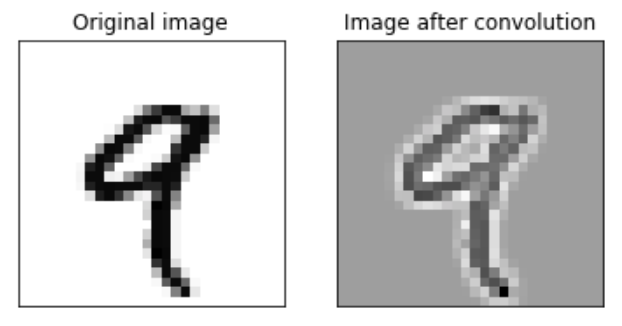
\includegraphics[width=10cm]{image_conv.png}
        \caption{Exemplo de convolução aplicada a uma imagem do dataset}
        \label{fig:img_conv}
\end{figure}

\begin{equation}
C_{3\times 3}= 
    \begin{bmatrix}
        -1 &-1 & -1  \\
        -1 &8 & -1  \\
        -1 &-1 & -1  \\
\end{bmatrix}
\label{eq:convEdge}
\end{equation}

A figura \ref{fig:img_conv} mostra um exemplo de convolução aplicada a uma imagem do datase. No Exemplo o filtro aplicado é descrito na matrix \ref{eq:convEdge}. Esse kernel é utilizado para evidenciar as bordas da imagem. 



\begin{table}[h!]
\centering
\begin{tabular}{l||l}

            &   Acurácia    \\ \hline
Treino      &   0.912           \\ \hline
Teste       &   0.904      
\\ \hline
Validação   &   0.902
\end{tabular}
\caption{Métricas obtidas no modelo gerado pela CNN}
  \label{tab:metrica_cnn}
\end{table}

A tabela \ref{tab:metrica_cnn} mostra como foi o desenpenho da CNN no dataset de treino, teste e validação. 

\begin{figure}[h!]
        \centering
        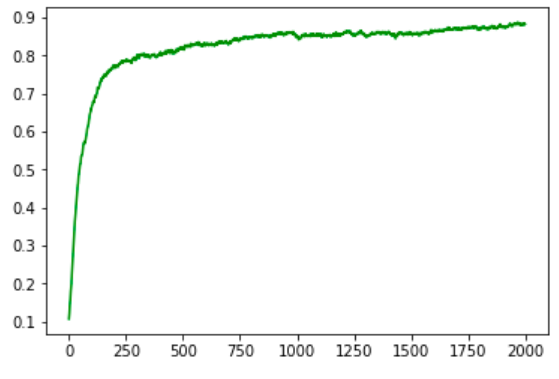
\includegraphics[width=10cm]{cnn_treinamento.png}
        \caption{Grafico da evolução da acurácia durante o treinamento}
        \label{fig:cnn_treinamento}
\end{figure}

A figuta \ref{fig:cnn_treinamento} mostra a evolução da acurácia da rede nos dados de teste ao longo das épocas. A etapa de treinamento é interrompida em 120 épocas após atingir 0.904 de acurácia.



\newpage

\bibliography{final_report}
\bibliographystyle{plain}
\end{document}

